\documentclass{article}

\usepackage[final]{project_nips_style}

% =========================
% Packages
% =========================
\usepackage[utf8]{inputenc}
\usepackage[T1]{fontenc}
\usepackage{hyperref}
\usepackage{url}
\usepackage{booktabs}
\usepackage{amsmath, amsfonts}
\usepackage{graphicx}
\usepackage{microtype}
\usepackage{xcolor}
\usepackage{float}

\usepackage{todonotes}


% =========================
% Title Information
% =========================
\title{Multimodal Skin Lesion Classification: Investigating the Influence of Metadata on Model Decision-Making}

\author{
  Eva Bauer \\
  University of Bern \\
  \texttt{eva.bauer@students.unibe.ch}
  \And
   Alexandra Benova \\
  University of Bern \\
  \texttt{alexandra.benova@students.unibe.ch}
   \And
   Nina Fröhlich \\
  University of Bern \\
  \texttt{nina.froehlich@students.unibe.ch}
}

\begin{document}

\maketitle


\vspace{0.5em}


% ============================================================
\section{Introduction and Background}
% ============================================================


Skin cancer is one of the most common cancer types worldwide, making early and accurate detection critical for effective treatment and reduced mortality risk \citep{watson2026, jerant2000early, dildar2021skin}. Diagnosis is often based on image analysis, which has led to the widespread use of deep learning models such as convolutional neural networks (CNNs) \citep{musthafa2024enhanced}.

More recently, multimodal approaches that combine image data with additional patient information have gained attention, as they provide a more comprehensive representation of clinical cases \citep{hao2025}. However, it remains unclear whether such models rely on clinically meaningful signals or instead exploit dataset-specific correlations present in metadata.

In this work, we investigate how patient metadata influences model decision-making in skin lesion classification by comparing image-only, metadata-only, and multimodal models. This setup allows us to assess the added value of incorporating complementary non-image information. However, performance metrics alone are not sufficient to explain the underlying decision-making mechanisms of the model. Therefore, in addition to analyzing the overall classification results, we investigate which metadata features contribute most strongly to the predictions and how the integration of metadata affects the model’s visual attention. 
We complement the quantitative performance analysis with explainability methods to better understand how the models reached their predictions.


% ============================================================
\section{Method}
% ============================================================ 

\subsection{Model Architectures}
We compare three architectures for binary skin lesion classification: an image-only ResNet18, a metadata-only TabTransformer, and a multimodal model combining both modalities.

\subsubsection{Image-Only Baseline}
For the image-only baseline we used a Resiudal Neural Network with 18 layers (ResNet18). ResNet employs residual skip connections, which facilitate the training of deeper networks by mitigating vanishing gradients~\cite{he2015deepresiduallearningimage}. 
We selected ResNet18 after it achieved the best validation performace on our dataset, in comparison to VGGNet and GoogLeNet. Further, this architecture is a commonly used approaches for skin lesion classification in literature \citep{7893267, yu2025ai, wu2022skin}.


%To establish a strong image-only baseline, we compared three widely used CNN architectures: VGGNet, GoogLeNet, and ResNet. These architectures were commonly used approaches for skin lesion classification in literature \citep{7893267, yu2025ai, wu2022skin}. Based on this comparison, we selected the best-performing architecture as the final image-only baseline for the remainder of the study.

%Further, we performed minor hyperparameter optimization, including adjustments to the learning rate and batch size to improve model performance. 
%Hyperparameter optimization was performed using Optuna with a Tree-structured Parzen Estimator sampler and a successive-halving pruning strategy. This was chosen instead of an exhaustive grid search because training multiple pretrained CNNs is computationally expensive, particularly on a small dataset. The pruning strategy allowed unpromising trials to be stopped early based on validation AUC, reducing the total training time. The search space included model architecture, learning rate, batch size, dropout, weight decay, and whether the pretrained backbone was frozen. Validation AUC was used as the optimization objective due to the binary and potentially imbalanced nature of the classification task.

\subsubsection{Metadata-Only Baseline}

For the metadata-only baseline, we used a TabTransformer, which embeds categorical variables as tokens and models feature interactions through self-attention~\cite{huang2020tabtransformer}. Numerical features were standardized, while categorical encodings were learned from the training set and reused for validation and testing.

In addition to serving as a strong standalone baseline, in literature this architecture is also as a metadata encoder for the multimodal models. Since the TabTransformer produces contextualised feature representations, it allows the metadata to be integrated more effectively with image features during multimodal fusion~\cite{sravani2025transformer}.

\subsubsection{Multimodal Model}

The multimodal model combines an image encoder and a metadata encoder into a joint classification framework, using the previous mentioned models.

The two modalities are fused using a cross-attention mechanism~\citep{cai2022multimodal}, where image features attend to the metadata representations. This allows the model to incorporate patient-level information into the visual feature space and condition predictions on both modalities. The fused representation is then passed to a classification head for final prediction. A conceptual overview is shown in Figure~\ref{fig:multimodal_architecture}.

In addition to enabling multimodal learning, the attention weights can be used to analyze how metadata features influence the model’s predictions, providing insight into the decision-making process.


%\subsection{Evaluation}

%Our evaluation was designed to address two main questions: whether the inclusion of patient metadata improves predictive performance, and how this additional information influences the model's decision-making process. 

%To assess predictive performance, we compared the image-only baseline, metadata-only baseline, and multimodal model on the binary classification task using standard metrics, including accuracy, precision, recall, F1-score, and area under receiver operating characteristic curve (AUROC). This comparison allowed us to determine whether combining image and metadata information provides an advantage over unimodal approaches.

%To investigate how metadata influences the decision process, we complemented the quantitative evaluation with explainability analyses. First, we examined the cross-attention weights of the multimodal model to identify which metadata features were emphasised for individual predictions. Second, we compared Grad-CAM visualisations of the image-only and multimodal models to analyze whether the inclusion of metadata affected the model's visual attention \citep{Selvaraju_2019}. Together, these analyses allowed us to study not only whether additional information improved classification performance, but also how it altered the model's internal decision-making behaviour.

%To test generalization of the three different models, we tested each of them on unseen data. For that we used the PAD-UFES-20 dataset.

\subsection{Training Setup}
\paragraph{Dataset} 
We used the MRA-MIDAS dataset~\citep{midas2023}, which contains dermoscopic and clinical images paired with patient metadata. Overall the dataset contains $3216$ images from $733$ patients, with $1500$ benign and $1419$ malignant labeled cases. The metadata contain patient-level information such as age, ethnicity, and sex, as well as lesion-specific attributes including size, anatomical location, and textual descriptions, and up to three additional clinical impressions per sample. Further information on the dataset distributions, such as patients age, skin lesion positions and a metadata correlation analysis, are presented in Fig.~\ref{fig:MIDASdataset_analysis}. 

\paragraph{Preprocessing}
In the preprocessing, we converted the ground-truth label into malignant and benign cases for binary classification. Samples without labels were excluded from the dataset. Further,the labeled data got split into training, validation, and test sets ($80\%$-$10\%$-$10\%$). To avoid data leakage, the dataset was split on a patient level.
%, ensuring that images from the same patient do not appear in multiple splits.

\paragraph{Implementation Details} 
% Loss function, Optimizer, Hyperparameters
Both the image-only as well as the multimodal model where trained using Binary Cross-entropy loss (BCEWithLogitsLoss), as it is a standard choice for modeling and evaluating predicted probabilities in binary classification tasks. A weight of positive examples was applied to adress class imbalance.\\
As an optimizer we choose AdamW because it combines an adaptive gradient-based optimization with regularization via a weight decay, leading to a stable training and improved generalization~\cite{loshchilov2019decoupledweightdecayregularization}.\\
All image encoders were initialized with ImageNet-pretrained weights.\\
Futher, we performend a hyperparameter optimization using Optuna, to determine optimal hyperparameter values for batch size, learning rate and weight decay. The selected hyperparameters are reported in Table~\ref{tab:Hyperopt}.\\
Training images were resized to $224 \times 224$ and augmented using random flips to increase the diversity of the training data and reduce overfitting. Additionally, the image-only model used rotation and color jitter. Those stronger augmentations were not applied to the multimodal to prevent a missmatch between image and metadata. Validation and test images were only resized and normalized.

\paragraph{Evaluation}
We evaluated all models using Area under Curver (AUC), balanced accuracy, and F1-score. Model behavior was analyzed using Grad-CAM and cross-attention weights to assess the influence of metadata on predictions.\\
To assess external generalization, we evaluated all models on a balanced subset of PAD-UFES-20 with $100$ benign and $100$ malignant samples~\cite{PACHECO2020103545}. 

%The dataset contains 3216 images from 733 patients, with 1500 benign and 1419 malignant labeled cases (for more information on the dataset see Figure~\ref{fig:MIDASdataset_analysis}).


%\subsection{Implementation Details}
%Mention practical decisions that affect results (initialization, regularization, augmentations, etc.).

%All image encoders were initialized with ImageNet-pretrained weights. Training images were resized to $224 \times 224$ and augmented using random flips to increase the diversity of the training data and reduce overfitting. Additionally, the image-only model used rotation and color jitter. Those stronger augmentations were not applied to the multimodal to prevent a missmatch between image and metadata. Validation and test images were only resized and normalized.\\

%Categorical metadata features were encoded and embedded, while numerical features were standardized using statistics fitted on the training set. Class imbalance was addressed with a weighted binary cross-entropy loss. Models were optimized with AdamW, and the best checkpoint was selected based on validation AUC. Early stopping was applied for the image-based models.



% ============================================================

\section{Results}

\subsection{Performance on MIDAS}

Table~\ref{tab:midas_results} summarizes the performance of the three implemented models. The TabTransformer achieves the best overall performance, with an AUC of $92\%$, indicating that the metadata contain highly informative features for the lesion classification. 

\begin{table}[H]
\centering
\caption{Performance of all models on the MIDAS dataset.}
\label{tab:midas_results}
\begin{tabular}{lccc}
\hline
\textbf{Model} & \textbf{Balanced Acc.} & \textbf{F1-score} & \textbf{AUC} \\
\hline

Image-only ResNet18 & 0.6703 & 0.6515 & 0.7678 \\
Metadata-only TabTransformer & 0.8253 & 0.8339 & \textbf{0.9158} \\
Multimodal ResNet18 & 0.7097 & 0.6694 & 0.7767 \\

\hline
\end{tabular}
\end{table}

In comparison, the image-only ResNet18 and the multimodal model show similar performance, with AUC values of $77\%$ and $78\%$, respectively. The multimodal model achieves a slightly higher balanced accuracy. This suggests that the inclusion of metadata provides a modest complementary benefit, although the overall improvement remains limited.

The comparatively lower performance of the image-based models may be attributed to the quality of the MIDAS images, which often contain substantial background noise and inconsistent cropping. This makes it more difficult for the model to identify the relevant lesion on the image.


\subsection{Explainability Evaluation}

The Grad-CAM heatmaps reveal that, in correctly predicted lesion images, both the image-only and multimodal models mainly focuse on the correct region in the image (Fig.~\ref{fig:grad_good}, \ref{fig:gradM_good}). However, when the image includes background elements or a black microscope frame, the area of interest shifts away from the lesion (Fig.~\ref{fig:grad_background}, ~\ref{fig:gradM_background}). In such cases, the confidence for correct predictions either decreases to just  above $50\%$ or the model fails to produce the correct prediction. The metadata importance plot of the multimodal (Fig.~\ref{fig:gradM_background}) indicated that, in these situations, metadata becomes more influential.

Furthermore, the Grad-CAM evaluation highlights that some false negatives occur because the model focuses on the wrong lesion. As illustrated in Fig.~\ref{fig:grad_lesion}, when images contain multiple lesions, the model tends to concentrate on a different lesion, which likely leads to incorrect predictions. 


%Grad-CAM visualizations showed that correctly classified images were generally associated with activation regions around the lesion. In contrast, misclassified samples more frequently exhibited attention on background regions or non-relevant structures, indicating that the model failed to localize the lesion reliably.

%This effect was particularly pronounced in images with substantial background clutter or black microscope frames, where the model’s attention often shifted away from the lesion area. Additionally, for patients with multiple images, predictions were more consistent when the lesion was clearly centered and well-cropped. When the lesion was poorly framed or less visible, the model’s confidence decreased, suggesting a reliance on clear and localized visual cues for accurate classification.

%Overall, these observations support the hypothesis that image quality and cropping inconsistencies significantly impact the performance of image-based models.

notes: FN to FN: multimodal model shifts often from the rigth lesion region to background




\subsection{Generalization to External Dataset}
As shown in Table~\ref{tab:pad_results}, the image-only model achieves improved performance on the external dataset. This is likely due to a higher image quality and more consistent lesion-centered cropping, which reduces background noise. This improved performes is also reflected in the multimodal model, which has the highest AUC of $89\%$. However, the metadata-only model performance significantly decreases. This is likely due to feature mismatch, as important MIDAS attributes such as race and ethnicity are not available in PAD-UFES-20. 
%The multimodal model achieved the best performance (AUC 0.8919), followed by the image-only model (AUC 0.8633). The metadata-only model performed close to random, indicating limited transferability of tabular features across datasets. This is likely due to feature mismatch, as important MIDAS attributes such as race and ethnicity are not available in PAD-UFES-20. 

\begin{table}[H]
\centering
\caption{Performance of all models on the PAD-UFES-20 dataset.}
\label{tab:pad_results}
\begin{tabular}{lccc}
\hline
\textbf{Model} & \textbf{Balanced Acc.} & \textbf{F1-score} & \textbf{AUC} \\
\hline

Image-only ResNet18 & 0.7450 & 0.7692 & 0.8633 \\
Metadata-only TabTransformer & 0.5150 & 0.5611 & 0.5143 \\
Multimodal ResNet18 & 0.8300 & 0.8350 & 0.8919 \\

\hline
\end{tabular}
\end{table}

% ============================================================




% ============================================================
\section{Conclusion}
% ============================================================
As our result show, including patient metadata in the decision-making process of a deep classification model improve performance. Especially in cases where the lesion is not the primary focus, metadata can be a determining factor in correctly classifying the lesion. 


\newpage
{\small
\bibliographystyle{unsrt}
\bibliography{references}
}

% ============================================================
\appendix
% ============================================================

\newpage
\section{Appendix (Optional)}

\subsection{Conceptual Overview}
\begin{figure}[H]
    \vspace{-2cm}
    \centering
    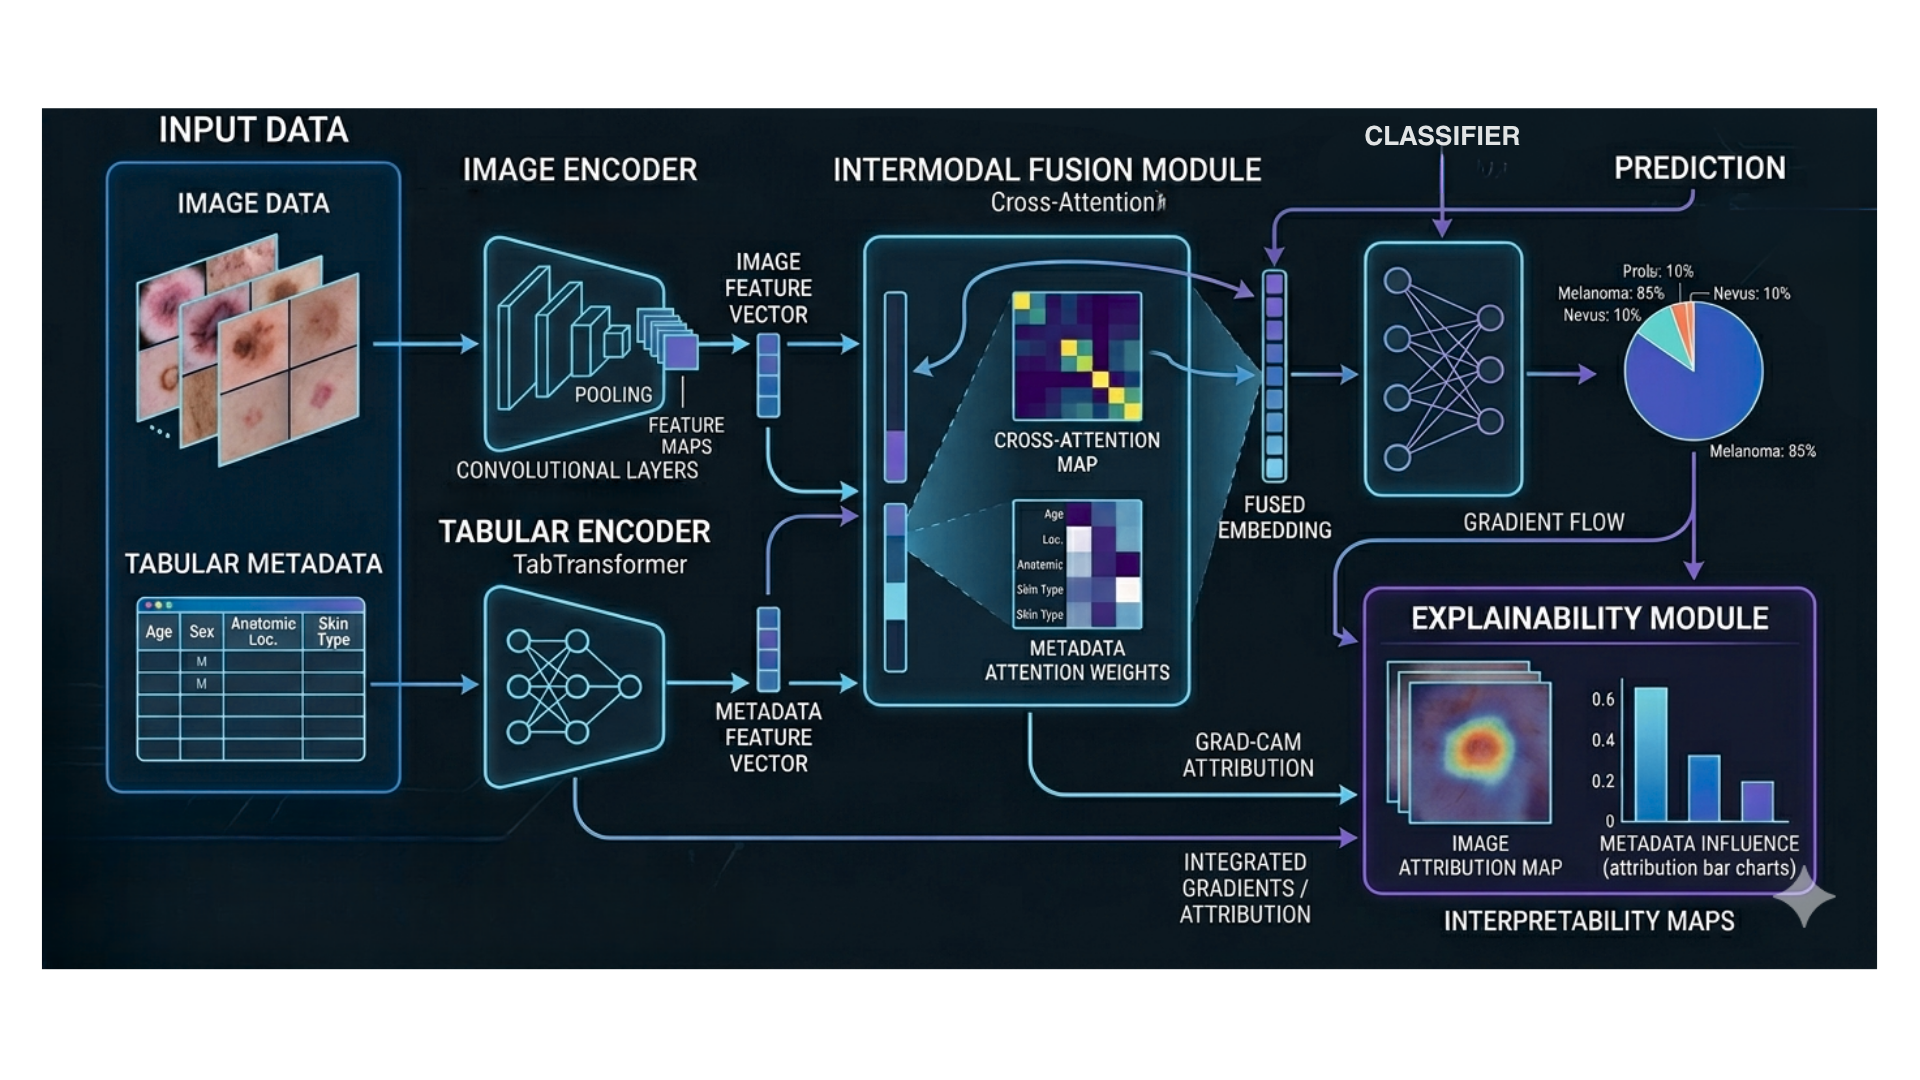
\includegraphics[width=\textwidth]{Img/multimodal_modal_setup.png}
    \caption{Conceptual overview of the proposed multimodal architecture. Skin lesion images are processed by a CNN-based image encoder, while patient metadata is encoded using a TabTransformer. Both representations are fused through a cross-attention module and passed to a classifier for final prediction. The architecture also facilitates interpretability by enabling analysis of visual attributions and metadata-related attention patterns. The figure was created with AI assistance and manually reviewed and adapted by the authors for technical accuracy.}
    \label{fig:multimodal_architecture}
\end{figure}

\subsection{Hyperparameter Results}
\begin{table}[h]
    \centering
    \caption{Chosen Hyperparameter for based on Optuna optimization}
    \begin{tabular}{lccc}
        \toprule
        \textbf{Model} & \textbf{Batch Size} & \textbf{Learning Rate} & \textbf{Weight Decay}\\
        \midrule
        ResNet18 & 32 & 4.38e-5 & 4.97e-5 \\
        \bottomrule
        \label{tab:Hyperopt}
    \end{tabular}
\end{table}

\subsection{MIDAS Dataset}
\begin{figure}[H]
    \centering
    
\includegraphics[width=\textwidth]{Img/midas_overview_figure.png}
    \label{fig:MIDASdataset_analysis}
    \caption{MIDAS Dataset Overview}
\end{figure}

\subsection{Confusion Matrix for Image-only Model}

\begin{table}[H]
\centering
\caption{Confusion matrix counts for the evaluated model.}
\label{tab:confusion_matrix}
\begin{tabular}{lc}
\hline
\textbf{Metric} & \textbf{Count} \\
\hline

True Positives (TP) & 89 \\
True Negatives (TN) & 100 \\
False Positives (FP) & 62 \\
False Negatives (FN) & 28 \\


\hline
\end{tabular}
\end{table}


\subsection{Performance metrics, if we want to use other/more}
\begin{table}[H]
\centering
\caption{Summary of model performance across evaluated settings.}
\label{tab:main_results_summary}
\begin{tabular}{llccccc}
\hline
\textbf{Model} & \textbf{Dataset} & \textbf{Accuracy} & \textbf{Precision} & \textbf{Recall} & \textbf{F1-score} & \textbf{AUC} \\
\hline

Image-only ResNet18 & MIDAS & 0.6703 & 0.5850 & 0.7350 & 0.6515 & \textbf{0.7678} \\
Metadata-only TabTransformer & MIDAS & 0.8253 & 0.7758 & 0.9014 & 0.8339 & 0.9158 \\
Multimodal ResNet18 & MIDAS & 0.7097 & 0.6406 & 0.7009 & 0.6694 & \textbf{0.7767} \\

Image-only ResNet18 & PAD-UFES-20 & 0.7450 & 0.7450 & 0.8500 & 0.7692 & 0.8633 \\
Metadata-only TabTransformer & PAD-UFES-20 & 0.5150 & 0.5124 & 0.6200 & 0.5611 & 0.5143 \\
Multimodal ResNet18 & PAD-UFES-20 & 0.8300 & 0.8113 & 0.8600 & 0.8350 & 0.8919 \\
\hline

\end{tabular}
\end{table}

\subsection{Grad-CAM Results}
\begin{figure}[H]
    \centering
    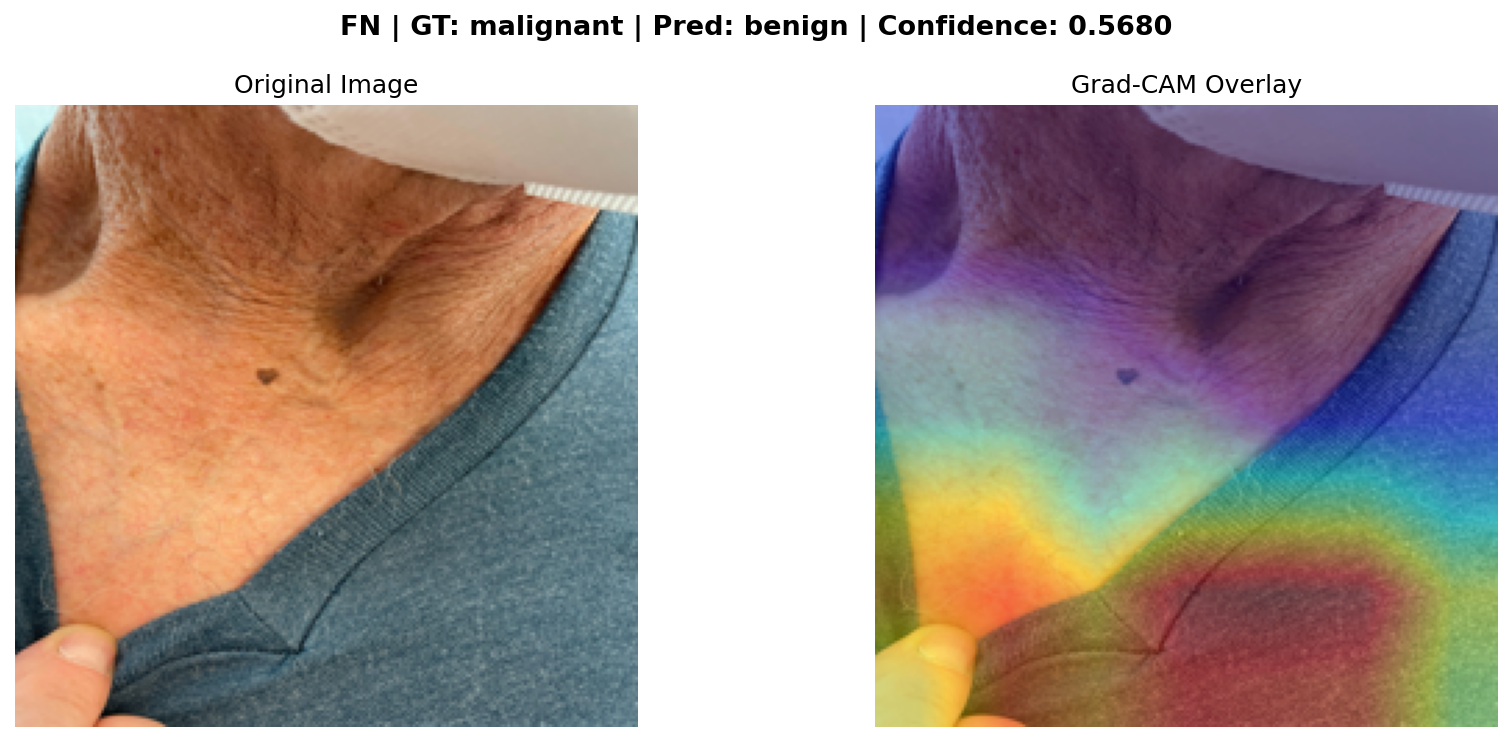
\includegraphics[width=\textwidth]{Img/FN_s-prd-663359577_gradcam.png}
    \caption{Background}
    \label{fig:grad_background}
\end{figure}

\begin{figure}[H]
    \centering
    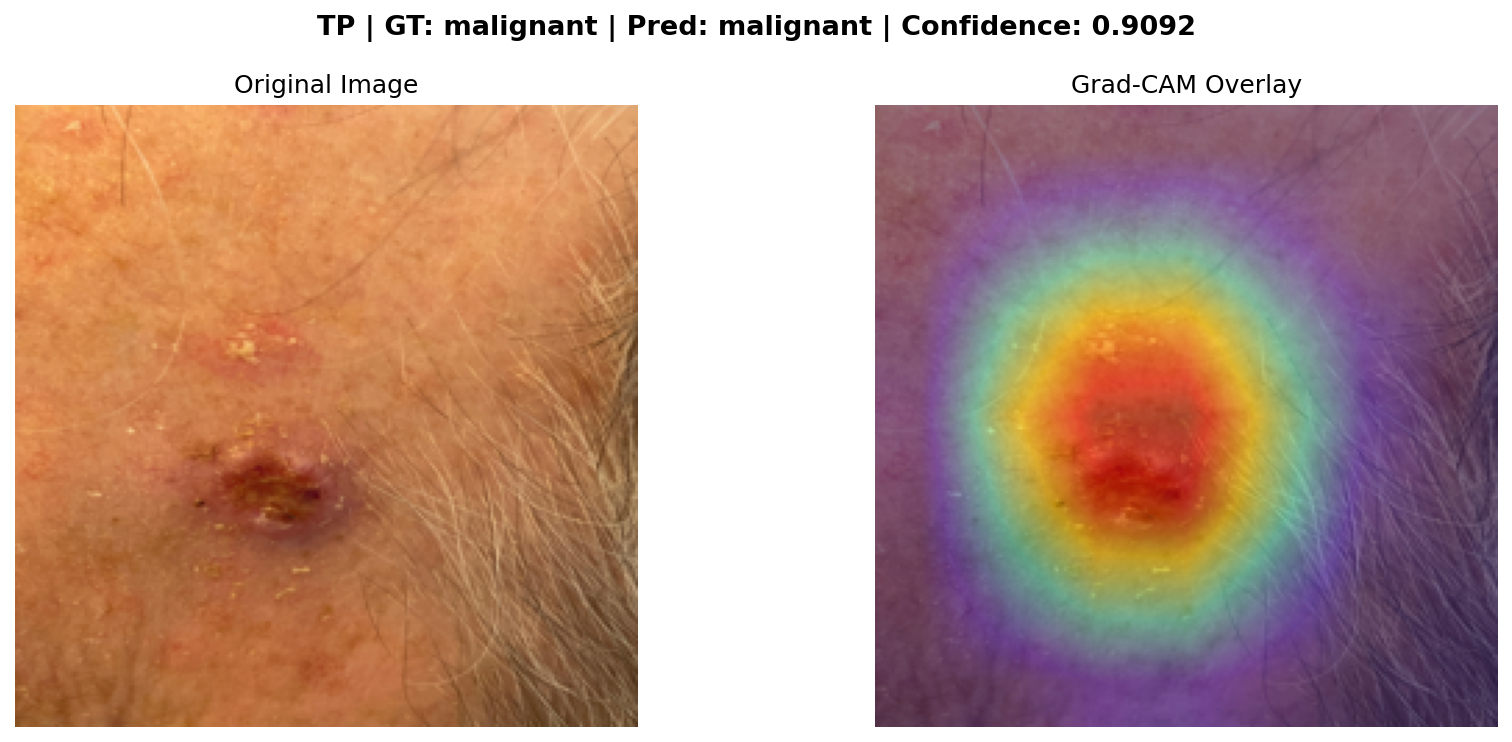
\includegraphics[width=\textwidth]{Img/TP_s-prd-759513907_gradcam.png}
    \caption{Good}
    \label{fig:grad_good}
\end{figure}

\begin{figure}[H]
    \centering
    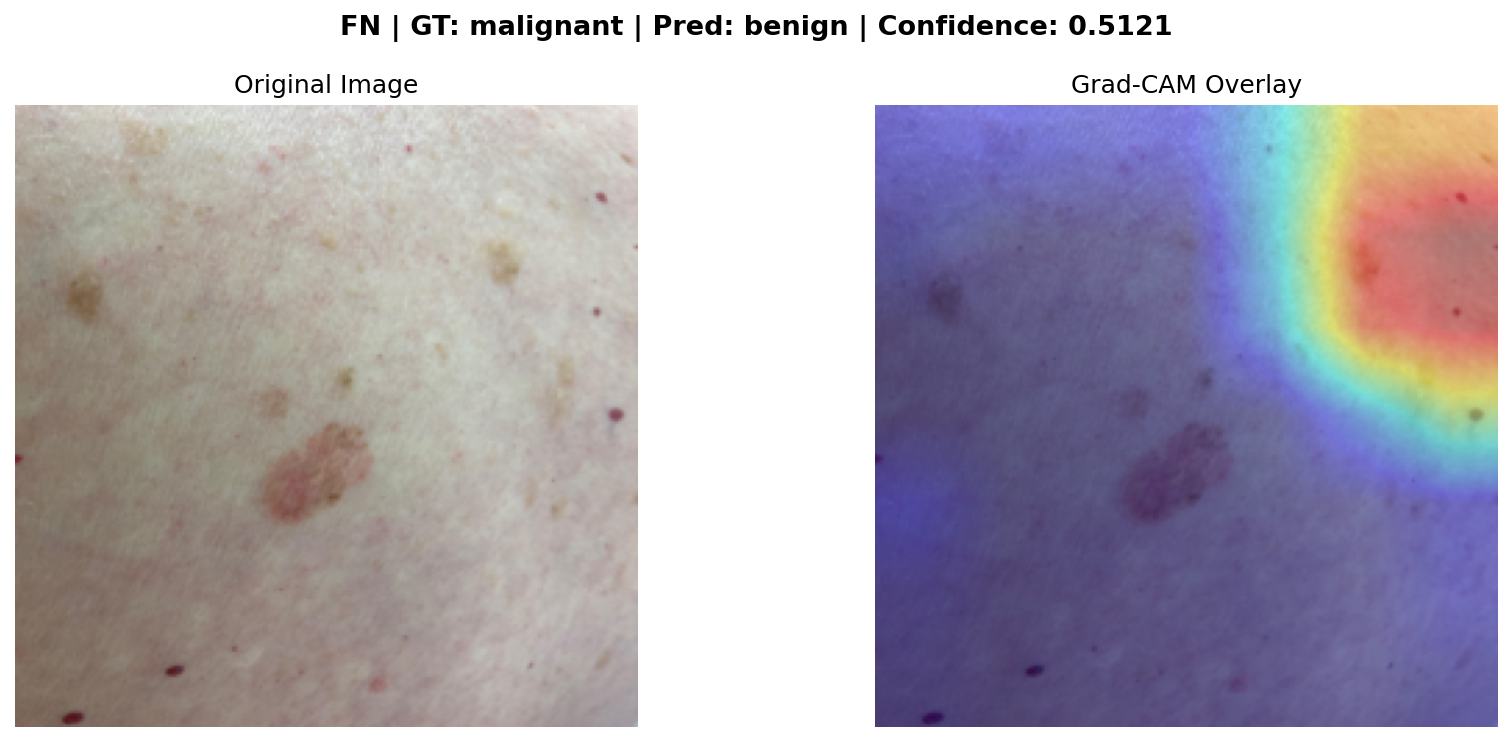
\includegraphics[width=\textwidth]{Img/FN_s-prd-762050418_gradcam.png}
    \caption{Wrong Lesion}
    \label{fig:grad_lesion}
\end{figure}

\begin{figure}[H]
    \centering
    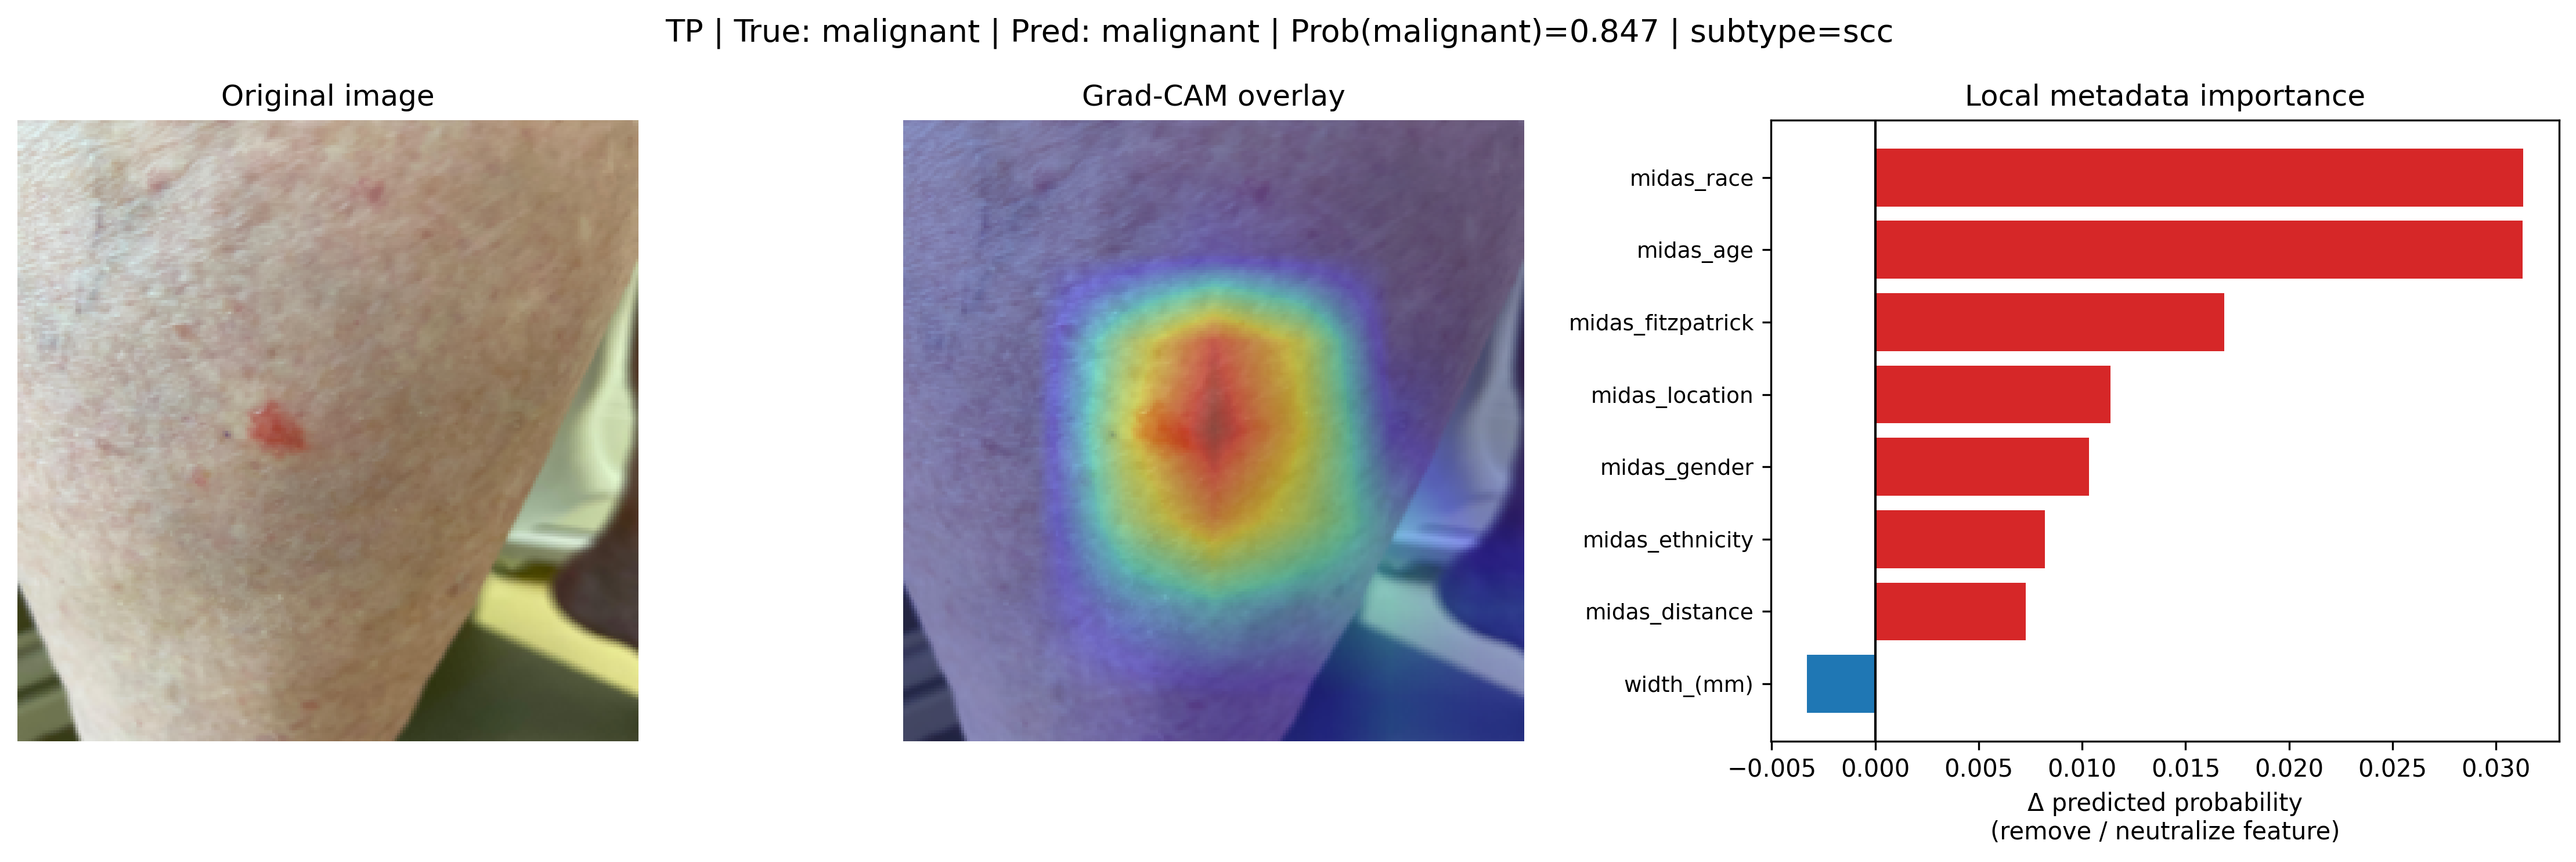
\includegraphics[width=\textwidth]{Img/TP_s-prd-499467412_p0.847.png}
    \caption{Good}
    \label{fig:gradM_good}
\end{figure}

\begin{figure}[H]
    \centering
    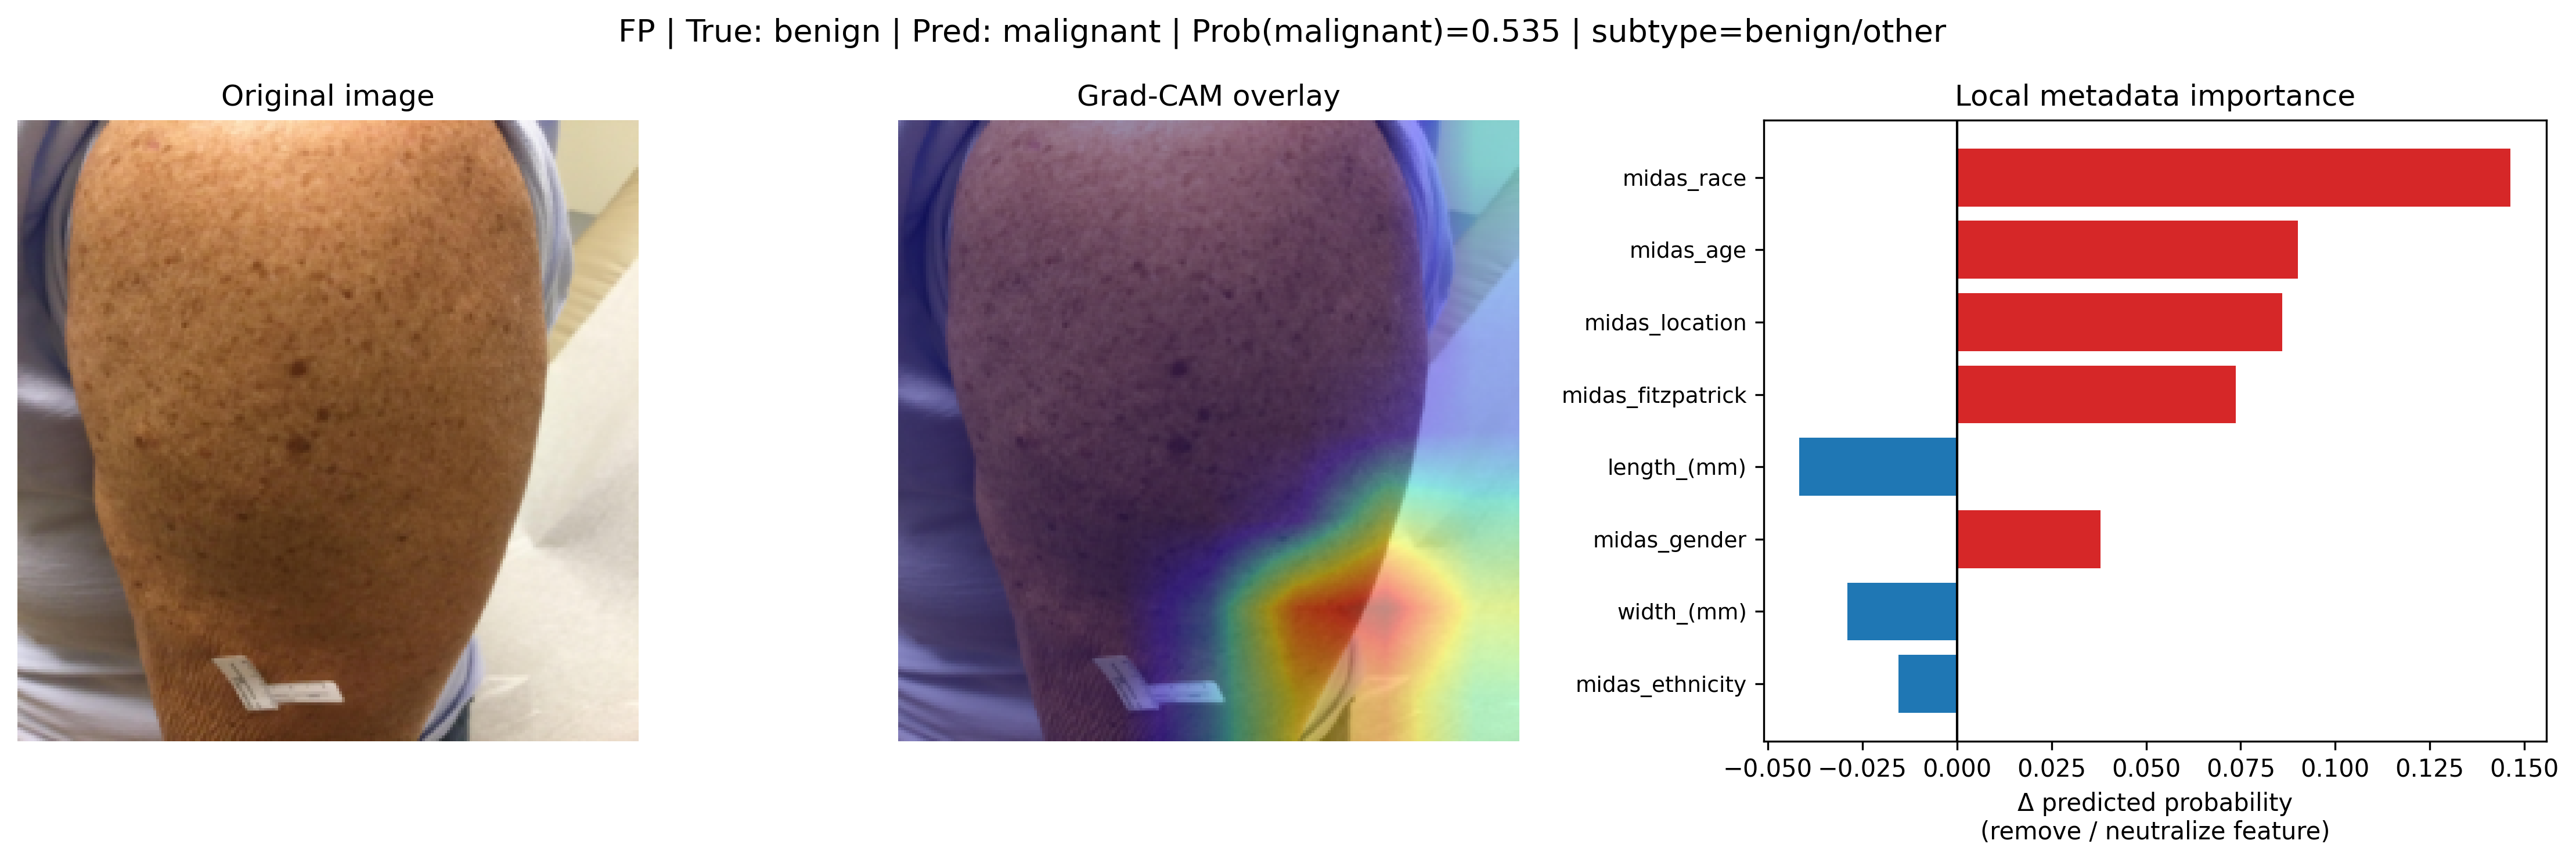
\includegraphics[width=\textwidth]{Img/FP_s-prd-725964889_p0.535.png}
    \caption{FP because of Background}
    \label{fig:gradM_background}
\end{figure}


\end{document}


